\chapter{関連研究}
\label{CRelatedWork}

%本研究で対象としている複眼の偽瞳孔現象をコンピュータグラフィックスの分野で扱った研究は未だ存在しない。
本研究では、複眼の偽瞳孔現象のビジュアライズを対象としている。
偽瞳孔は複眼表面の微細構造によって巨視的に現れる模様\figref{FWhatIsPseudopupil}であり、偽瞳孔をコンピュータグラフィックスの分野で扱った研究はあまり存在しない。
しかしながら、複眼同様に表面の微細構造を有している材質などのレンダリングを扱った研究は少なからず存在するため、それらを紹介し、本研究との比較を行う。

\section{微細構造を扱った研究}
\label{SMicrostructure}

表面微細構造をもつ物質をレンダリングする研究が過去にいくつか行われている。
本節では、マイクロファセットモデル、構造色、織布のレンダリングに関する研究をそれぞれ簡略して紹介する。

\subsection{マイクロファセットモデル}

表面のマイクロファセット(microfacet)構造の例として車の塗装のようにざらついたようなきらめきを持つ材質がある。
こうした材質をレンダリングする手法として、G\"{u}ntherら\cite{guenther05efficientacquisition}はノーマルマップ(normal map: 法線マップ)を利用し、Rumpら\cite{rump-2008-photo-realistic}は測定したテクスチャを用いた手法をそれぞれ提唱している。

%Guenther
\begin{figure}[htbp]
 \begin{minipage}{0.4\hsize}
  \begin{center}
   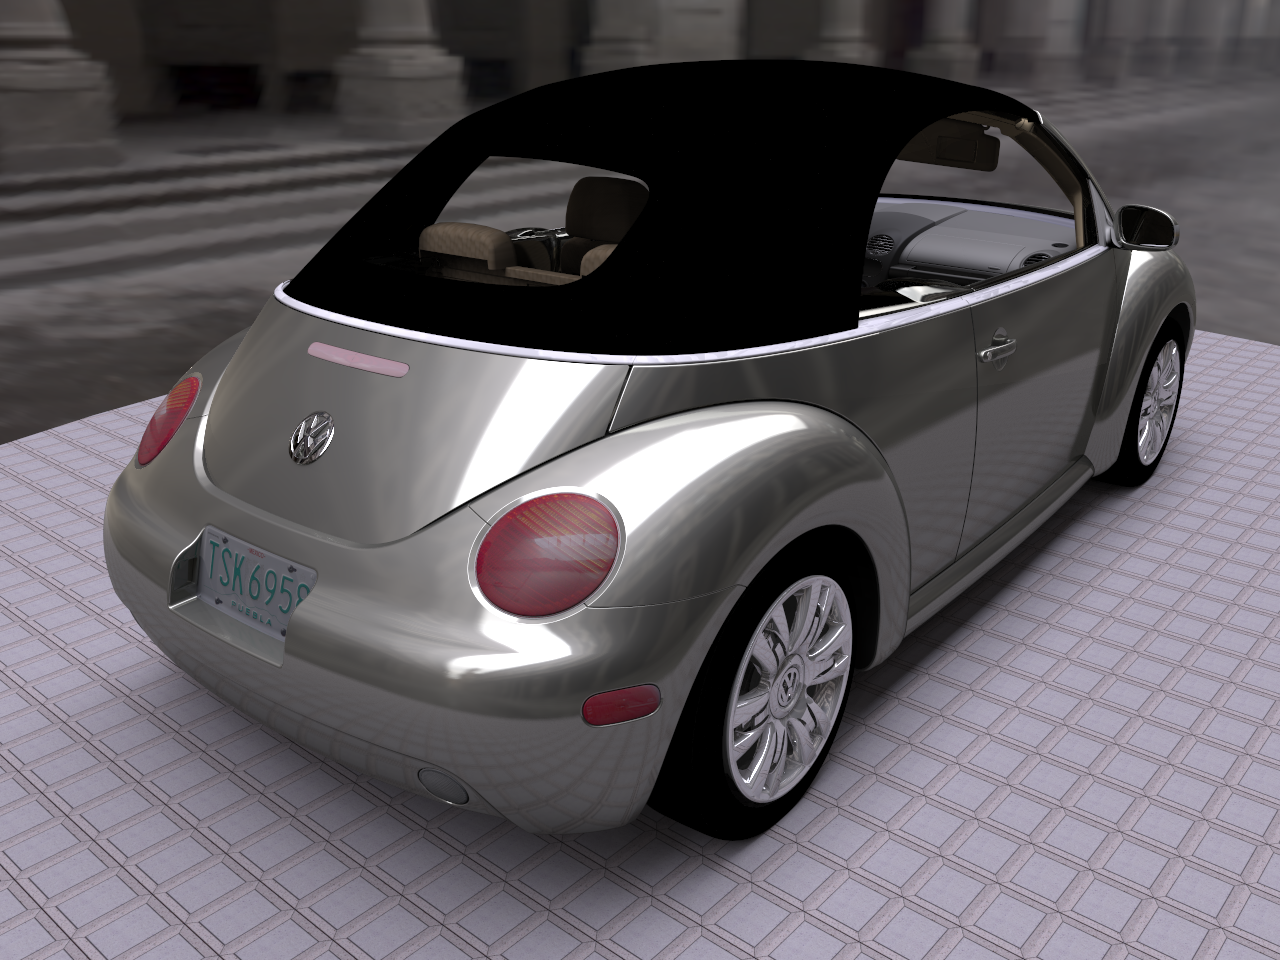
\includegraphics[width=70mm]{./img/back_hq.png}
  \end{center}
  \caption{G\"{u}nther1}
  \label{FGuenther1}
 \end{minipage}
 \begin{minipage}{0.75\hsize}
  \begin{center}
    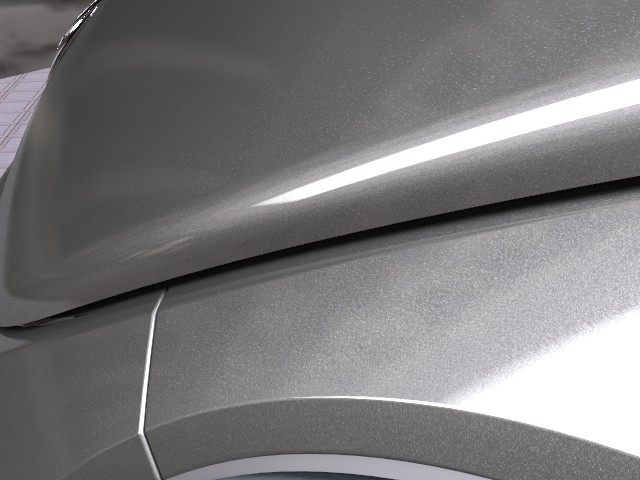
\includegraphics[width=70mm]{./img/sparkles.png}
  \end{center}
  \caption{G\"{u}nther2}
  \label{FGuenther2}
 \end{minipage}
\end{figure}

%Rump
\begin{figure}[htbp]
 \begin{minipage}{0.4\hsize}
  \begin{center}
   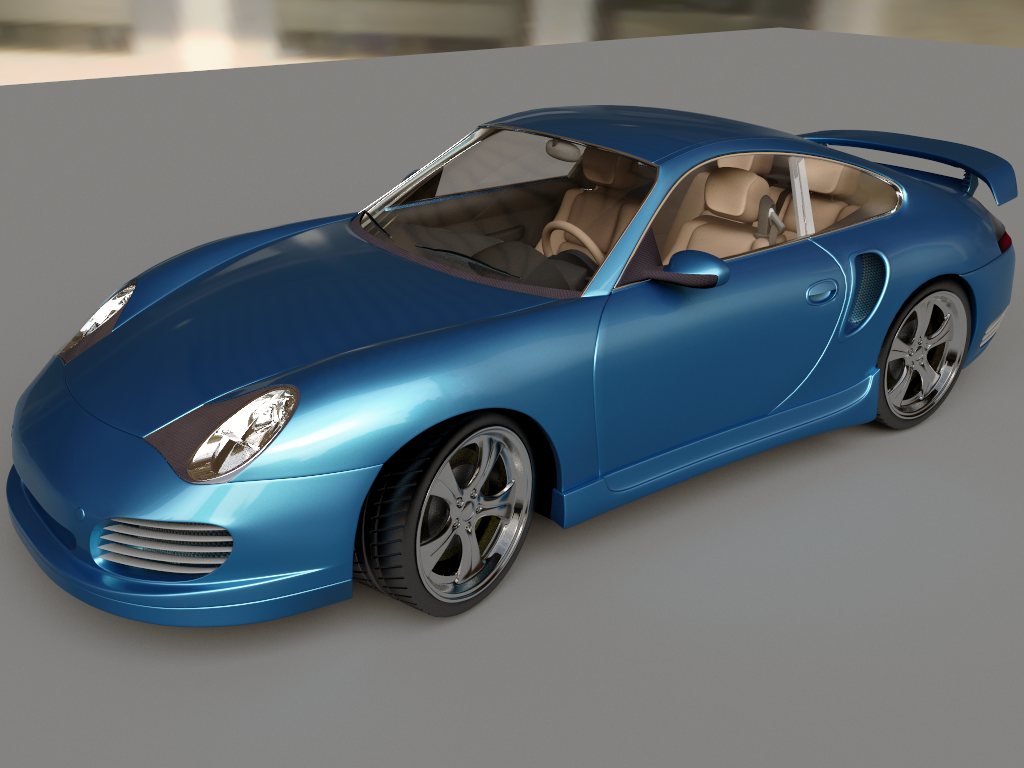
\includegraphics[width=70mm]{./img/porsche01.png}
  \end{center}
  \caption{Rump1}
  \label{FRump1}
 \end{minipage}
 \begin{minipage}{0.75\hsize}
  \begin{center}
    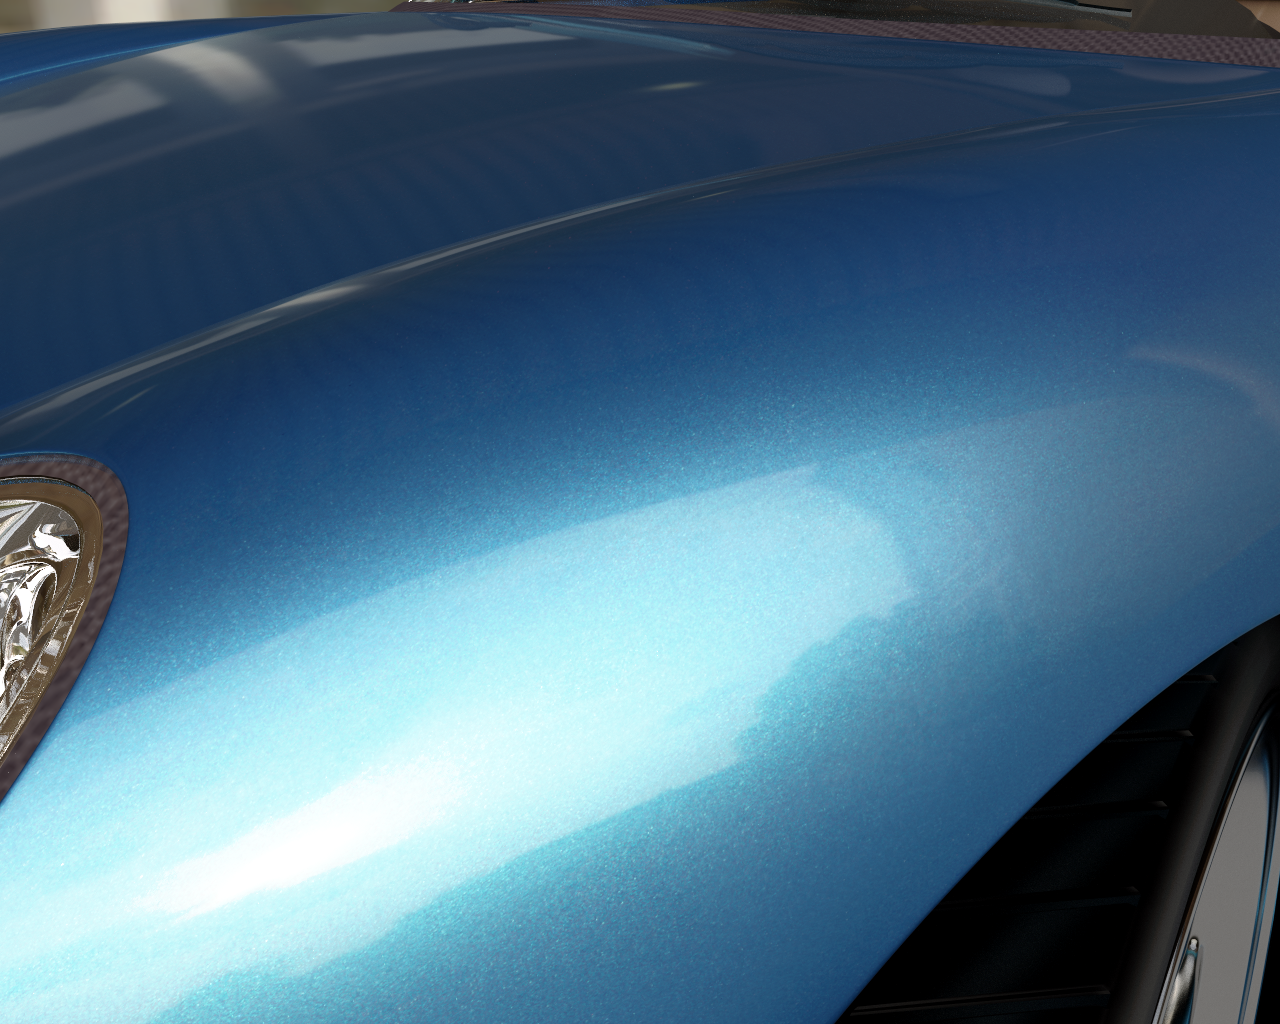
\includegraphics[width=70mm]{./img/porsche03.png}
  \end{center}
  \caption{Rump2}
  \label{FRump2}
 \end{minipage}
\end{figure}

\noindent
また、Jakobら\cite{jakob2014discrete}の行ったハイヒールの表面やクリスマスオーナメント\figref{FHeelOrnament}のようにきらめく材質のレンダリングに関する研究では、サーフェスもしくは観測者の動きに合わせて変化するきらめきのランダムなパターンを表現している。
この手法の対象は鏡のような薄片を含むダイナミックにきらめく表面材質、およびかすかに小さいスケールのきらめきを示す粗い表面材質である。
これらの現象は原則的にはG\"{u}ntherらのように高解像度のノーマルマップによって表現することができる。
しかし、細かな特徴をもつマップは角度のついた照明条件下ではエイリアシング(aliasing)において重大な問題を抱えてしまう。
それゆえ、Jakobらは通常では連続しているマイクロファセットの分布をサーフェス上の離散的な散乱粒子の分布と置き換えた、確率論的なモデルを提唱している。
この確率論的な階層では、個別の粒子を考えることなく多数のランダムな粒子の存在下で効率的な評価を行うことができ、それによってマルチスケールにおいて双方向反射率分布関数(BRDF: Bidirectional Reflectance Distribution Function)を導くことができる。

\begin{figure}[hn]
  \centering
  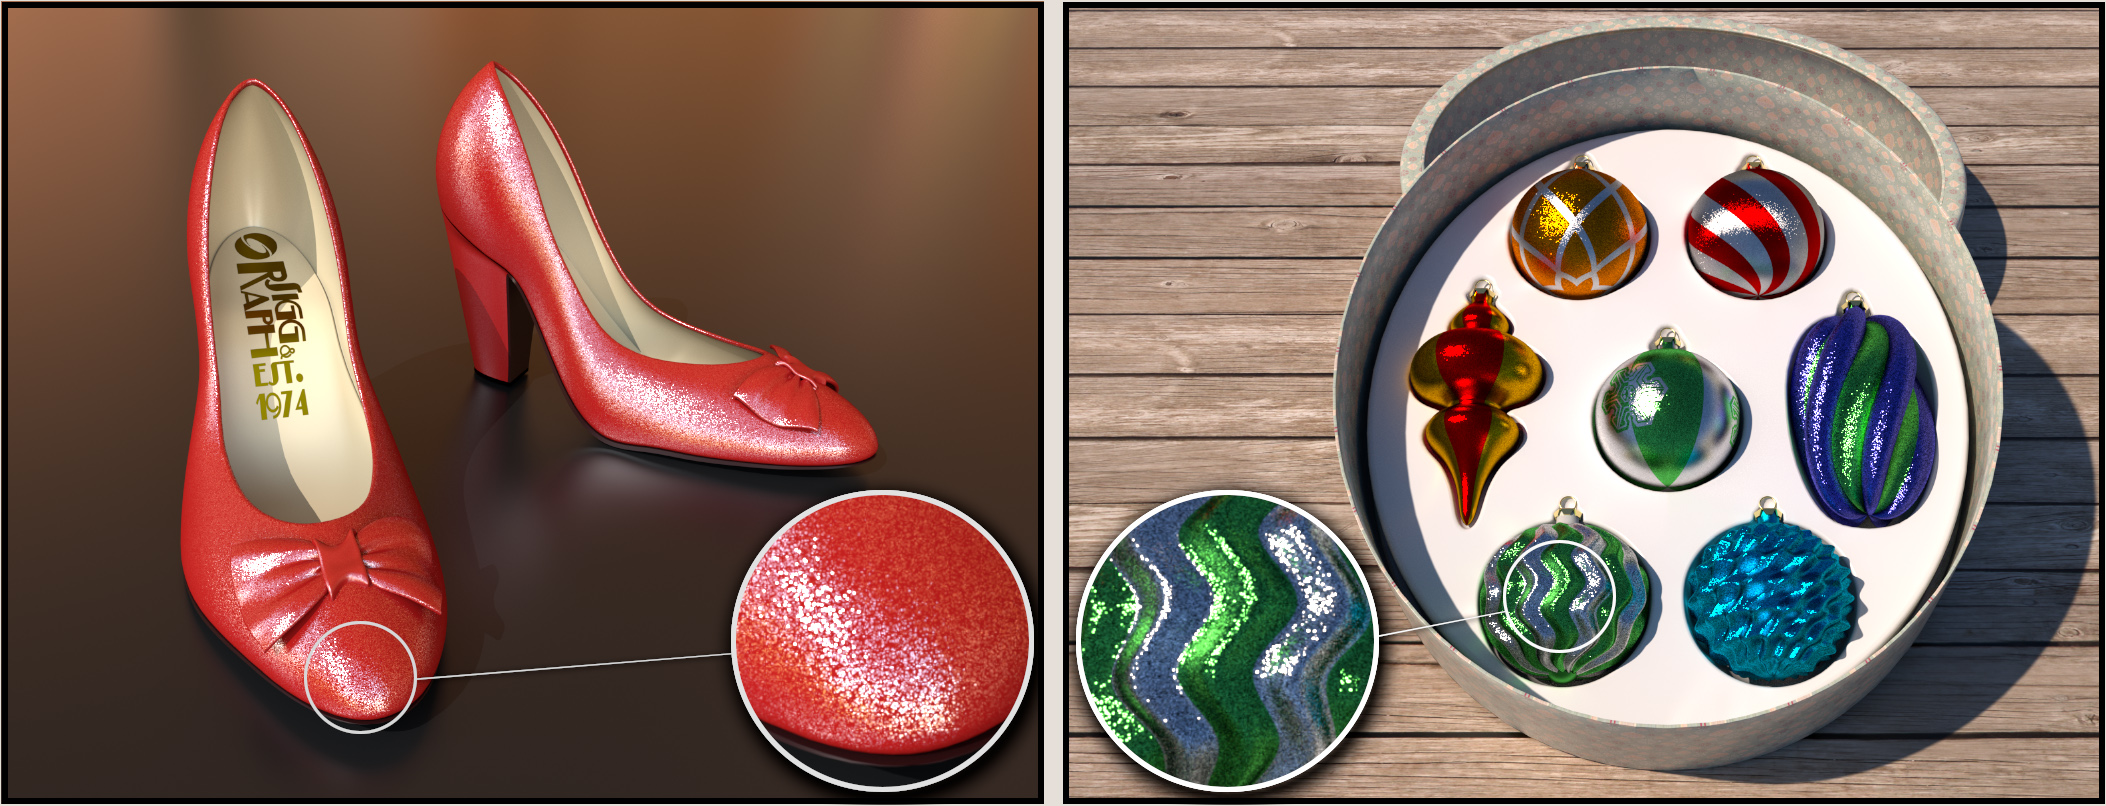
\includegraphics[width=5.0in]{./img/heel_ornament.jpg}
  \caption{ハイヒールとオーナメント(\cite{jakob2014discrete}より転載)}
  \label{FHeelOrnament}
\end{figure}


\subsection{構造色CG}

\begin{figure}[htbp]
  \centering
  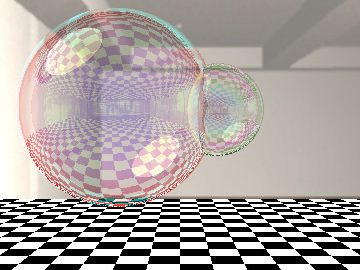
\includegraphics[width=3.5in]{./img/syabon_iwasaki.jpg}
  \caption{シャボン玉の薄膜干渉(\cite{iwasaki2004real}より転載)}
  \label{FSyabon}
\end{figure}

\begin{figure}[htbp]
  \centering
  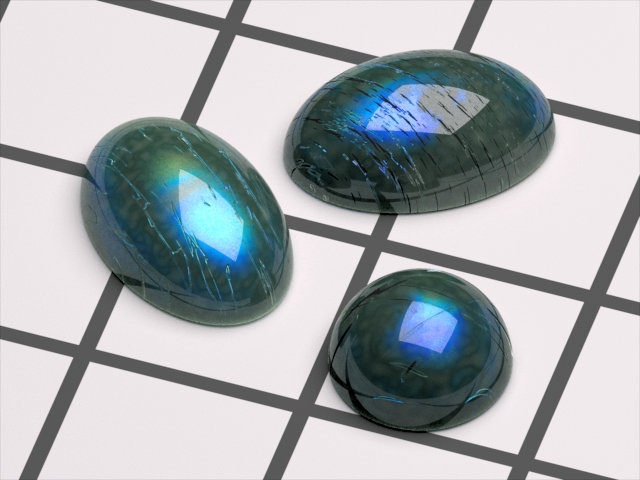
\includegraphics[width=3.5in]{./img/kouseki_weidlich.jpg}
  \caption{鉱石の多層膜干渉(\cite{weidlich2009rendering}より転載)}
  \label{FKouseki}
\end{figure}

普段、人間が知覚する色の多くは色素によるものであり、光の吸収や反射によって色として認識される。
一方、構造色は光の干渉による強弱や、光の散乱などによって起こる現象である。
そのため、媒質の屈折率が変化すると色素による色は変化しないが構造色は変化するなどの特徴がある。

こうした性質のある構造色をCGで表現する研究は1980年代にはすでに行われており、現在に至るまでさまざまな物質や気象現象に関する構造色がCGによって表現されている。
その中でも、とくに物体の表面構造が関係している構造色の例としては、薄膜干渉によるシャボン玉\figref{FSyabon}や多層膜干渉による鉱石\figref{FKouseki}、回折によって生じるCDなどの光学ディスク、そのほかにも鱗粉のミクロ構造によるモルフォチョウの翅などが挙げられる。

たとえば、シャボン玉の表面は薄膜構造になっており厚みが光の波長以下となるため、薄膜の表面で反射する光と薄膜の裏面で反射する光が干渉を起こし虹色に見える。
Icartら\cite{icart1999approach}は重力による薄膜の厚みの変化を考慮したシャボン玉のCG表現の研究を行い、岩崎ら\cite{iwasaki2004real}は薄膜の厚みが動的に変化するシャボン玉をレンダリングする研究を行い、事前計算によるテクスチャを生成することによってリアルタイムでの表現を可能とした。
これらのように、形状などのジオメトリの変化が色に変化を与えることも構造色の特徴である。
また、多層膜のように干渉する膜の数が増えると、光の計算はさらに複雑になる。

%% \textcolor{red}{****回折、モルフォの解説****}

\begin{figure}[htbp]
  \centering
\subfigure[岩澤の手法(\cite{iwasawa2004rendering}より転載)]{
\includegraphics*[width=.75\columnwidth]{./img/morpho_s.jpg}
\label{FMorpho1}}\\
\subfigure[Sadeghiの手法(\cite{sadeghi2008physically}より転載)]{
\includegraphics*[width=.45\columnwidth]{./img/Morpho_sadeghi.png}
\label{FMorpho2}}
\subfigure[岡田の手法(\cite{okada2013rendering}より転載)]{
\includegraphics*[width=.45\columnwidth]{./img/morpho_okada.jpg}
\label{FMorpho3}}
  \caption{様々な手法によるモルフォチョウのレンダリング}
  \label{FMorpho}
\end{figure}

\newpage
\subsection{織布のレンダリング}

織布は織糸の小さいスケールの立体構造によって変化するさまざまな外観を有する。
その構造的なディティールを正確にモデリングすることで非常にリアリスティックな織布のレンダリングをすることができるが、織糸レベルのボリューメトリック(volumetric)なモデルを作成するには非常にコストがかかる。

Zhaoら\cite{zhao2012structure}は織糸の立体構造を自由に構築するために、詳細な生地サンプルをスキャンするのではなく、シンプルな織り構造の生地サンプルをスキャンすることによってボリューメトリックな標本のデータベースを作成し、それらからデータをコピーすることによって目的のボリュームデータを合成している。
その結果、統一的にさまざまな織りの布を表現することができ、大小のスケールの両方で非常にリアルな出力画像を生み出すことができている。

%% \textcolor{red}{****もう少し解説を追加****}

\begin{figure}[htbp]
 \begin{minipage}{0.4\hsize}
  \begin{center}
   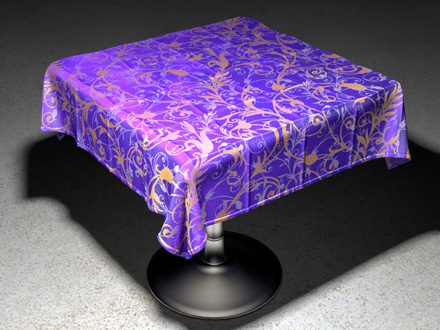
\includegraphics[width=70mm]{./img/mft_purple_cloth_ld.jpg}
  \end{center}
  \caption{織布のレンダリング(\cite{zhao2013modular}より転載)}
  \label{FZhao1}
 \end{minipage}
 \begin{minipage}{0.75\hsize}
  \begin{center}
    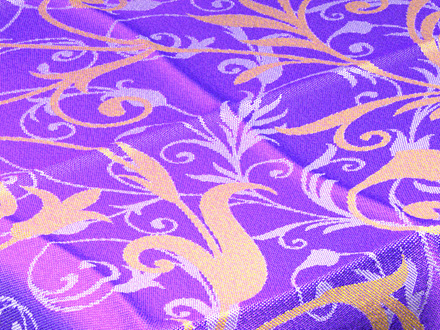
\includegraphics[width=70mm]{./img/mft_zoom_ld.jpg}
  \end{center}
  \caption{織布のレンダリング(拡大)(\cite{zhao2013modular}より転載)}
  \label{FZhao2}
 \end{minipage}
\end{figure}

\begin{figure}[htbp]
  \centering
  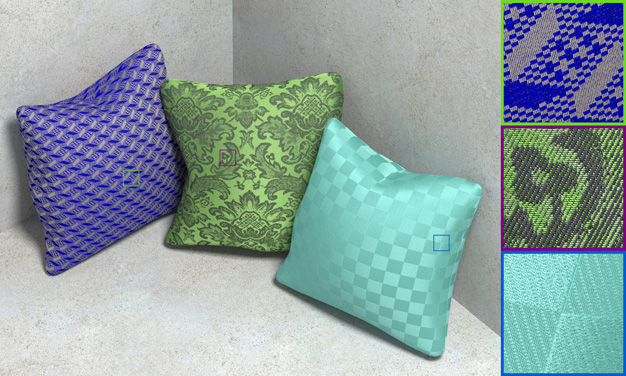
\includegraphics[width=5.5in]{./img/cussions.jpg}
  \caption{織布のレンダリング(\cite{zhao2012structure}より転載)}
  \label{FZhao3}
\end{figure}

\section{本研究の位置づけ}
\label{SPosition}

先述のように、表面微細構造を考慮したレンダリングに関する研究はいくつか存在する。
それらは本研究で対象としている複眼のCG表現と直接的に関連する研究ではないが、いずれも微細な構造が巨視的な外観に影響する材質に関する研究であると言える。
マイクロファセットおよび構造色は肉眼では視認できない微細な構造をしている一方、織布のレンダリングに関しては、肉眼で目視可能なレベルのスケールの構造物があり、複眼と同様に一定の条件で整列した構造をしている。
また、こうした微細構造に基づく質感は品質を要求するほど計算時間がかかるため、両立することが困難な場合がある。
本研究では、微細構造をもつ複眼をの外観に対してリアリティを追求しつつ、リアルタイム処理の実現を目標とする。


%% \textcolor{red}{****比較とか****}
%% \textcolor{red}{ほかのやつはたいていランダムにやってもできるけど、本研究の対象である複眼は綺麗に並んでるやつだからそう簡単にはいかないよ}
